\chapter{物理内存管理}\label{ch_memory}

\section{本章概要}

\paragraph{一句话描述}
在现代计算系统中,软件所在的代码和数据都是在内存中处理的,操作系统需要管理好内存,让代码和数据能够合理放置在相关位置;且通过提供动态申请内存和释放内存的功能,让自己和依靠操作系统的应用能够灵活高效地使用内存。


\paragraph{概述}

一个编程人员希望拥有容量无限大、速度无限快,而且是非易失型的(nonvolatile)的内存空间,到lab1为止,这个梦想还无法轻易满足。为此绝大多数的计算机采用了一种折衷的方法,即建立一个分层的存储器结构,最高层是CPU内部的一些寄存器,它们的访问速度是最快的,但容量不是很大,一般小于1KB;第二层是高速缓存(即硬件cache),实现在CPU内部,接近寄存器速度,容量一般小于4MB;第三层是主存储器(内存),其访问速度比寄存器小一个数量级、价格便宜,目前几百块人民币就可以买到4GB。以上这三种存储器都是易失型的,即在断电后,其内容全部会丢失掉。第四层是磁盘,它的访问速度较慢、价格较便宜,目前花几百块钱就可以买到存储容量\textgreater{}1TB的硬盘,而且是非易失型的。

操作系统需要尽量满足编程人员的梦想,为此它需要管理上述存储器层次结构形成的存储空间,并完成如下主要任务:

\begin{itemize}
	\item
	记录存储空间的使用情况,即记录哪些部分正在被使用,哪些部分还空闲;
	\item
	当需求方需要存储空间时,能快速地分配给它合适大小的空间;在需求方显式表示不需要申请到的存储空间时,能把存储空间回收,便于以后的分配;
	\item
	隔离不同的内存区域,确保在限制在一个内存区域中运行的软件无法访问区域以外的内存空间。这种机制称为地址保护(地址隔离)机制。
	\item
	如果内存太小,就需要把内存当中使用较少的数据所占空间送到磁盘上,给使用较多的数据腾出内存空间来;如果将来又访问到缓存到硬盘的数据,需要把这些数据重新加载到内存中进行访问。这种机制称为换入换出(swap
	in/out)机制,并涉及页替换算法。
	\item
	即使需求方表明了需要内存,但如果需求方没有实际访问所需内存前,则并不完成实际的物理内存分配。这种机制称为按需分配(如果是基于很分页机制,也称为按需分页)。
	\item
	设两个具有父子关系的程序共享同一地址空间(子程序同享父程序的地址空间),若二程序只是读此地址空间,则地址空间不会有变化;若其中一个程序对此地址空间某地址进行了写操作,则要把包含此地址的页空间复制一份给执行写操作的程序,这时此二程序将有不同的地址空间,可独立运行,相互不干扰。这种机制减少了父程序创建子程序地址空间的开销,称为写时复制(Copy
	On Write,简称COW)机制。
\end{itemize}

\paragraph{本章涉及的实验}

本章内容主要涉及操作系统的内存管理,包括物理内存管理和基于分页机制的虚拟内存管理。读者通过阅读本章的内容并动手实践相关的5个project实验:

\begin{itemize}
	\item
	proj5:能够探测物理内存并建立页表,实现分页管理
	\item
	proj5.1/5.1.1/5.1.2:实现基于连续物理页的first/best/worst-fit分配算法
	\item
	proj5.2:实现基于连续物理页的buddy分配算法
	\item
	proj6:实现任意大小内存分配的slab分配算法
	\item
	proj7:实现缺页中断服务例程和虚拟内存管理结构(VMM
	struct),提供按需分页的支持
	\item
	proj8:实现类似改进时钟算法的页面置换算法并支持页粒度的换入换出机制
	\item
	proj9/proj9.1/proj9.2:完善虚存管理(proj9)并逐步实现了进程间内存共享(proj9.1)和copy
	on write(COW)机制(proj9.2)
\end{itemize}



\paragraph{本章收获的知识}

\textbf{可以掌握如下知识:} * 与操作系统原理相关 *
内存管理:基于分页机制的内存管理 * 内存管理:连续内存分配算法 *
内存管理:非连续内存分配算法 * 内存管理和中断:缺页中断服务例程 *
内存管理:虚存管理中的页面置换算法和页换入换出机制 *
内存管理:按需分页机制和写时复制机制 * 操作系统原理之外 *
80386对分页管理(页表等)的硬件支持 *
页粒度的页面置换策略和页换入换出的具体实现

本章内容中主要涉及内存管理的重要功能主要有两个:

\begin{itemize}
\item
  提供空闲内存空间:这样给操作系统和应用程序的代码和数据足够的存放``地方'',使得二者能够正常高效地运行,为此需要完成内存/外存的空间的分配、管理、释放等算法。
\item
  提供内存空间隔离保护:隔离用户态应用程序和内核态操作系统之间,以及不同应用程序之间的内存空间,使得不会出现访问冲突,为此需要为不同的应用程序和操作系统划分不同的地址空间,一个应用程序越界规定的地址空间会出现内存访问故障中断。
\end{itemize}

为了让读者能够从实践上来理解内存管理的基本原理,我们设计了上述实验,主要的功能逐步实现如下所示:
* 首先是扩展ucore的功能,使它能够发现并管理PC系统中可用的空闲物理内存;
*
然后是建立分页机制,建立线性地址(分段机制已经完成了逻辑地址到线性地址的转换)到物理地址的映射关系和具体转换操作,这样使得应用程序无法直接访问到物理地址,而是只能访问由操作系统设定好的物理地址空间,从而使得应用程序的访问空间可控;
*
为了高效地完成操作系统的其他功能单元和应用程序的空闲内存空间需求,需要设计以页(4096字节)为最小分配单位的面向连续物理地址空间的内存分配算法;
还要设计面向任意大小的内存空间(在物理地址空间上不一定连续)的虚拟内存分配算法;
*
为了给应用程序提供超过实际物理内存空间大小的虚拟内存空间,需要把临时不常用到的内存换出(swap
out)到硬盘(也称外存)中,等到需要访问的时候,再换入(swap
in)到内存中。设计高效的页面置换算法会尽量保存经常访问的数据在内存中,而不经常访问的数据会换出到硬盘中。

\section{试验目标}\label{ux8bd5ux9a8cux76eeux6807}

操作系统和应用程序都需要内存空间来存放代码和数据,这要求操作系统能够高效管理和保护整个计算机中的物理内存,并给自己和上层应用提供简洁安全的内存申请和释放的服务接口。通过分段机制可以完成虚拟地址到线性地址的转换,而通过分页机制可以进一步完成线性地址到物理地址的转换。分段机制中对每段的大小是可变的,分页机制中页的大小固定为4KB,这样在操作系统对实现内存管理上会更加简洁。所以在建立好分页机制后,分段机制的映射功能退化为对等映射,即虚拟地址=线性地址,这样实际的地址映射工作将由分页机制来完成。

为此ucore需要在已有的分段机制的基础上,进一步加入分页机制,达到可以通过分页完成对不同应用程序执行的内存空间进行隔离(其实分段也能够达到此目的,但相对实现的开销会比较大,受到的限制(比如支持的应用执行个数)也较多)的目标。并且为后续的虚存管理提供基础支持。

\section{proj5/5.1/5.1.1/5.1.2/5.2概述}\label{proj55.15.1.15.1.25.2ux6982ux8ff0}

\subsection{实现描述}\label{ux5b9eux73b0ux63cfux8ff0}

proj5基于proj4.3实现,主要完成了对计算机实际物理内存大小与分布的探测,实现以页(大小为4KB)为单位的简单物理内存管理,并通过建立二级页表,实现了分页内存管理,为将来试验中实现虚存管理打下一个基础。通过分析和实现proj5,读者可以了解到:
* 物理内存空间布局的探测; * 基于分页机制的存储管理; *
32位地址空间的二级页表结构;

proj5.1在proj5的基础上实现了基于best
fit内存分配算法的页级内存分配和释放功能;proj5.1.1在proj5.1的基础上实现了first
fit内存分配算法的页级内存分配和释放功能;proj5.1.2在proj5.1的基础上实现了worst
fit内存分配算法的页级内存分配和释放功能;proj5.2在proj5.1的基础上实现了更加实用和强大的buddy内存分配算法的页级内存分配和释放功能。这些proj是操作系统原理相关算法的具体实现。读者可以参考这些实现完成新的内存分配算法。在这里通过讲解proj5的实现,让读者理解如何基于一个内存分配管理框架来实现不同的内存分配算法。

\subsection{项目组成}\label{ux9879ux76eeux7ec4ux6210}

\begin{lstlisting}
proj5
|-- boot
|   |-- asm.h
|   |-- bootasm.S
|   `-- bootmain.c
|-- kern
|   |-- init
|   |   |-- entry.S
|   |   `-- init.c
|   |-- mm
|   |   |-- default_pmm.c
|   |   |-- default_pmm.h
|   |   |-- memlayout.h
|   |   |-- mmu.h
|   |   |-- pmm.c
|   |   `-- pmm.h
|   |-- sync
|   |   `-- sync.h
|   `-- trap
|       |-- trap.c
|       |-- trapentry.S
|       |-- trap.h
|       `-- vectors.S
|-- libs
|   |-- atomic.h
|   |-- list.h
`-- tools
    |-- kernel.ld
\end{lstlisting}

相对与proj4.3,proj5增加了6个文件。主要修改和增加的文件如下: *
boot/bootasm.S:增加了对计算机系统中物理内存布局的探测功能; *
kern/init/entry.S:根据临时段表重新暂时建立好新的段空间,为进行分页做好准备。
*
kern/mm/default\_pmm.{[}ch{]}:提供基本的基于链表方法的物理内存管理(分配单位为页,即4096字节);
*
kern/mm/pmm.{[}ch{]}:pmm.h定义物理内存管理类框架struct~pmm\_manager,基于此通用框架可以实现不同的物理内存管理策略和算法(default\_pmm.{[}ch{]}
实现了一个基于此框架的简单物理内存管理策略);~pmm.c包含了对此物理内存管理类框架的访问,以及与建立、修改、访问页表相关的各种函数实现。
*
kern/sync/sync.h:为确保内存管理修改相关数据时不被中断打断,提供两个功能,一个是保存eflag寄存器中的中断屏蔽位信息并屏蔽中断的功能,另一个是根据保存的中断屏蔽位信息来使能中断的功能;
*
libs/list.h:定义了通用双向链表结构以及相关的查找、插入等基本操作,这是建立基于链表方法的物理内存管理(以及其他内核功能)的基础。其他有类似双向链表需求的内核功能模块可直接使用list.h中定义的函数。
*
libs/atomic.h:定义了对一个变量进行读写的原子操作,确保相关操作不被中断打断。
* tools/kernel.ld:修改了ucore的起始入口和代码段的起始地址

\subsection{编译运行}\label{ux7f16ux8bd1ux8fd0ux884c}

编译并运行proj5的命令如下:

\begin{lstlisting}
make
make qemu
\end{lstlisting}

则可以得到如下显示界面

\begin{lstlisting}
chenyu@chenyu-laptop:~/oscourse/ucore-svn/lab2_memory/proj5$ make qemu
(THU.CST) os is loading ...

Special kernel symbols:
  entry  0xc010002c (phys)
  etext  0xc010537f (phys)
  edata  0xc01169b8 (phys)
  end    0xc01178dc (phys)
Kernel executable memory footprint: 95KB
memory managment: default_pmm_manager
e820map:
  memory: 0009f400, [00000000, 0009f3ff], type = 1.
  memory: 00000c00, [0009f400, 0009ffff], type = 2.
  memory: 00010000, [000f0000, 000fffff], type = 2.
  memory: 07efd000, [00100000, 07ffcfff], type = 1.
  memory: 00003000, [07ffd000, 07ffffff], type = 2.
  memory: 00040000, [fffc0000, ffffffff], type = 2.
check_alloc_page() succeeded!
check_pgdir() succeeded!
check_boot_pgdir() succeeded!
-------------------- BEGIN --------------------
PDE(0e0) c0000000-f8000000 38000000 urw
  |-- PTE(38000) c0000000-f8000000 38000000 -rw
PDE(001) fac00000-fb000000 00400000 -rw
  |-- PTE(000e0) faf00000-fafe0000 000e0000 urw
  |-- PTE(00001) fafeb000-fafec000 00001000 -rw
--------------------- END ---------------------
++ setup timer interrupts
100 ticks
100 ticks
……
\end{lstlisting}

通过上图,我们可以看到ucore在显示其entry(入口地址)、etext(代码段截止处地址)、edata(数据段截止处地址)、和end(ucore截止处地址)的值后,探测出计算机系统中的物理内存的布局(e820map下的显示内容)。接下来ucore会以页为最小分配单位实现一个简单的内存分配管理,完成二级页表的建立,进入分页模式,执行各种我们设置的检查,最后显示ucore建立好的二级页表内容,并在分页模式下响应时钟中断。下面我们将分析到底发生了什么事情。

\section{【背景】探测计算机系统中的物理内存分布和大小}\label{ux80ccux666fux63a2ux6d4bux8ba1ux7b97ux673aux7cfbux7edfux4e2dux7684ux7269ux7406ux5185ux5b58ux5206ux5e03ux548cux5927ux5c0f}

在proj5中,操作系统需要知道了解整个计算机系统中的物理内存如何分布的,哪些被可用,哪些不可用。其基本方法是通过BIOS中断调用来帮助完成的。其中BIOS中断调用必须在实模式下进行,所以在bootloader进入保护模式前完成这部分工作相对比较合适。这些部分由boot/bootasm.S中从probe\_memory处到finish\_probe处的代码部分完成完成。通过BIOS中断获取内存可调用参数为e820h的INT
15h BIOS中断。BIOS通过系统内存映射地址描述符(Address Range
Descriptor)格式来表示系统物理内存布局,其具体表示如下:

\begin{lstlisting}
Offset  Size    Description     
00h    8字节   base address               #系统内存块基地址
08h    8字节   length in bytes            #系统内存大小
10h    4字节   type of address range  #内存类型
\end{lstlisting}

看下面的(Values for System Memory Map address type) Values for System
Memory Map address type:

\begin{lstlisting}
01h    memory, available to OS
02h    reserved, not available (e.g. system ROM, memory-mapped device)
03h    ACPI Reclaim Memory (usable by OS after reading ACPI tables)
04h    ACPI NVS Memory (OS is required to save this memory between NVS sessions)
other  not defined yet -- treat as Reserved
\end{lstlisting}

INT15h BIOS中断的详细调用参数:

\begin{lstlisting}
eax:e820h:INT 15的中断调用参数;
edx:534D4150h (即4个ASCII字符“SMAP”) ,这只是一个签名而已;
ebx:如果是第一次调用或内存区域扫描完毕,则为0。 如果不是,则存放上次调用之后的计数值;
ecx:保存地址范围描述符的内存大小,应该大于等于20字节;
es:di:指向保存地址范围描述符结构的缓冲区,BIOS把信息写入这个结构的起始地址。
\end{lstlisting}

此中断的返回值为:

\begin{lstlisting}
cflags的CF位:若INT 15中断执行成功,则不置位,否则置位; 
eax:534D4150h ('SMAP') ;
es:di:指向保存地址范围描述符的缓冲区,此时缓冲区内的数据已由BIOS填写完毕 
ebx:下一个地址范围描述符的计数地址 
ecx :返回BIOS往ES:DI处写的地址范围描述符的字节大小 
ah:失败时保存出错代码
\end{lstlisting}

这样,我们通过调用INT 15h
BIOS中断,递增di的值(20的倍数),让BIOS帮我们查找出一个一个的内存布局entry,并放入到一个保存地址范围描述符结构的缓冲区中,供后续的ucore进一步进行物理内存管理。这个缓冲区结构定义在memlayout.h中:

\begin{lstlisting}
struct e820map {
    int nr_map;
    struct {
        long long addr;
        long long size;
        long type;
    } map[E820MAX];
};
\end{lstlisting}


\section{【实现】物理内存探测}\label{ux5b9eux73b0ux7269ux7406ux5185ux5b58ux63a2ux6d4b}

物理内存探测是在bootasm.S中实现的,相关代码很短,如下所示:

\begin{lstlisting}
probe_memory:
//对0x8000处的32位单元清零,即给位于0x8000处的
//struct e820map的结构域nr_map清零
    movl $0, 0x8000     
    xorl %ebx, %ebx    
//表示设置调用INT 15h BIOS中断后,BIOS返回的映射地址描述符的起始地址
    movw $0x8004, %di 
start_probe:
    movl $0xE820, %eax // INT 15的中断调用参数
//设置地址范围描述符的大小为20字节,其大小等于struct e820map的结构域map的大小
    movl $20, %ecx  
//设置edx为534D4150h (即4个ASCII字符“SMAP”),这是一个约定
    movl $SMAP, %edx
//调用int 0x15中断,要求BIOS返回一个用地址范围描述符表示的内存段信息
    int $0x15
//如果eflags的CF位为0,则表示还有内存段需要探测
    jnc cont
//探测有问题,结束探测
    movw $12345, 0x8000
    jmp finish_probe
cont:
//设置下一个BIOS返回的映射地址描述符的起始地址
    addw $20, %di
//递增struct e820map的结构域nr_map
    incl 0x8000
//如果INT0x15返回的ebx为零,表示探测结束,否则继续探测
    cmpl $0, %ebx
    jnz start_probe
finish_probe:
\end{lstlisting}

上述代码正常执行完毕后,在0x8000地址处保存了从BIOS中获得的内存分布信息,此信息按照struct
e820map的设置来进行填充。这部分信息将在bootloader启动ucore后,由ucore的page\_init函数来根据struct
e820map的memmap(定义了起始地址为0x8000)来完成对整个机器中的物理内存的总体管理。

\section{【原理】分页内存管理}\label{ux539fux7406ux5206ux9875ux5185ux5b58ux7ba1ux7406}

在分页内存管理中,一方面把实际物理内存(也称主存)划分为许多个固定大小的内存块,称为物理页面,或者是页框(page
frame);另一方面又把CPU(包括程序员)看到的虚拟地址空间也划分为大小相同的块,称为虚拟页面,或者简称为页面、页(page)。页面的大小要求是2的整数次幂,一般在256个字节到4M字节之间。在本书中,页面的大小设定为4KB。在32位的86x86中,虚拟地址空间是4GB,物理地址空间也也是4GB,因此在理论上程序可访问到1M个虚拟页面和1M个物理页面。软件的每一物理页面都可以放置在主存中的任何地方,分页系统(需要CPU等硬件系统提供相应的分页机制硬件支持,详见下一节)提供了程序中使用的虚地址和主存中的物理地址之间的动态映射。这样当程序访问一个虚拟地址时,支持分页机制的相关硬件自动把CPU访问的虚拟地址虚拟地址拆分为页号(可能有多级页号)和页内偏移量,再把页号映射为页帧号,最后加上页内偏移组成一个物理地址,这样最终完成对这个地址的读/写/执行等操作。

假设程序在运行时要去读地址0x100的内容到寄存器1(用REG1表示)中,执行如下的指令:

\begin{lstlisting}
mov 0x100, REG1
\end{lstlisting}

虚拟地址0x100被发送给CPU内部的内存管理单元(MMU),然后MMU通过支持分页机制的相关硬件逻辑就会把这个虚拟地址是位于第0个虚拟页面当中(设页大小为4KB),页内偏移是0x100;而操作系统的分页管理子系统已经设置好第0个虚拟页面对应的是第2个物理页帧,物理页帧的起始地址是0x2000,然后再加上页内的偏移地址0x100,所以最后得到的物理地址就是0x2100。然后MMU就会把这个真正的物理地址发送到计算机系统中的地址总线上,从而可正确访问相应的物理内存单元。

如果操作系统的分页管理子系统没有设置第0个虚拟页面对应的物理页帧,则表示第0个虚拟页面当前没有对应的物理页帧,这会导致CPU产生一个缺页异常,由操作系统的缺页处理服务例程来选择如何处理。如果缺页处理服务例程认为这是一次非法访问,它将报错,终止软件运行;如果它认为是一次合理的访问,则它会采用分配物理页等手段建立正确的页映射,使得能够重新正确执行产生异常的访存指令。

% rv_pages_hardware

\section{【背景】X86的分页硬件支持}\label{ux80ccux666fx86ux7684ux5206ux9875ux786cux4ef6ux652fux6301}

X86
CPU对实际物理内存的访问是通过连接着CPU和北桥芯片的前端总线来完成的,在前端总线上传输的内存地址是物理内存地址。物理内存地址被北桥映射到实际的内存条中的内存单元相应位置上。然而,在CPU内执行带来软件所使用的是虚拟内存地址(也称逻辑内存地址),它必须被转换成物理地址后,才能用于实际内存访问。

前面已经讲过了80x86的分段机制,80x86的分页机制建立在其分段机制基础之上,提供了更加强大的内存管理支持。需要注意的是,在x86中,必须先有分段机制,才能有分页机制。在分段机制中,虚地址会转换为线性地址。如果不启动分页机制,那么线性地址就是最终在前端总线上的物理地址;如果启动了分页机制,则线性地址还会经过页映射被转换为物理地址。

那如果启动分页机制呢?在80x86中有一个CR0控制寄存器,它包含一个PG位,如果PG=1,启用分页机制;如果
PG=0,禁用分页机制。不像分段机制管理大小不固定的内存卡,分页机制以固定大小的存储块为最小管理单位,即把整个地址空间(包括线性地址和物理地址)都看成由固定大小的存储块组成。在80x86中,这个固定大小一般设定为4096字节。在线性地址空间中的最小管理单位(称为页(page)),可以映射到物理地址空间中的任何一个最小管理单位(称为页帧(page
frame))。页/页帧的32位地址由20位的页号/页帧号和12位的页/页帧内偏移组成。

80x86分页机制中的分页转换功能(即线性地址到物理地址的映射功能)需采用驻留在内存中的数组来描述,该数组称为页表(page
table)。每个数组项就是一个页表项。由于页/页帧基地址按4096字节对齐,因此页/页帧的基地址的低12位是0。页地址\textless{}-\textgreater{}页帧地址的转换过程以简单地看做80x86对页表的一个查找过程。页地址(线性地址)的高20位(即页号,or页的基地址)构成这个数组的索引值,用于选择对应页帧的页帧号(即页帧的基地址)。页地址的低12位给出了页内偏移量,加上对应的页帧基地址就最终形成对应的页帧地址(即物理地址)。

由于80x86的地址空间可达到4GB,按页大小(4KB)划分为1M个页。如果用一个页表来描述这种映射,那么该也表就要有1M个表项,若每个表项占用4个字节,那么该映射表就要占用4M字节。考虑到将来一个进程就需要一个地址映射表,若有多个进程,那地址映射表所占的总空间将非常巨大。为避免地址映射表占用过多的内存资源,80x86把地址映射表设定为两级。地址映射表的第一级称为页目录表,存储在一个4KB的物理页中,页目录表共有1K个表项,其中每个表项为4字节长,页表项中包含对应第二级表所在的基地址。地址映射表的第二级称为页表,每个页表也安排在一个4K字节的页中,每张页表中有1K个表项,每个表项为4字节长,包含对应页帧的基地址。由于页目录表和页表均由1K个表项组成,所以使用10位的索引就能指定表项,即用10位的索引值乘以4加基地址就得到了表项的物理地址。按上述的地址转换描述,一个页表项只需20位,但实际的页表项是32位,那其他的12位有何用途呢?

在80x86中的的页目录表项结构定义如下所示:

\begin{figure}[htbp]
\centering
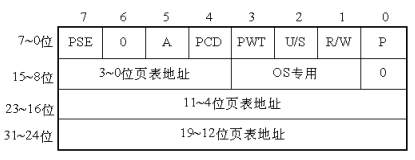
\includegraphics{figures/1.png}
\caption{1}
\end{figure}

在80x86中的的页表项结构定义如下所示:

\begin{figure}[htbp]
\centering
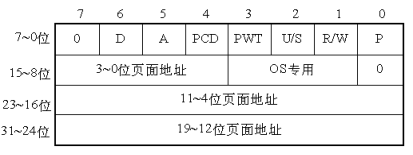
\includegraphics{figures/2.png}
\caption{2}
\end{figure}

其中低12位的相应属性位含义如下:

\begin{itemize}
\item
  P位:存在(Present)标志,用于指明此表项是否有效。P=1表示有效;P=0表示无效。如果80x86访问一个无效的表项,则会产生一个异常。如果P=0,那么除表示表项无效外,其余位用于其他用途(比如swap
  in/out中,用来保存已存储在磁盘上的页面的序号)。
\item
  R/W:读/写(Read/Write)标志,如果R/W=1,表示页的内容可以被读、写或执行。如果R/W=0,表示页的内容只读或可执行。当处理器运行在特权级(级别0、1或2)时,则R/W位不起作用。
\item
  U/S:是用户态/特权态(User/Supervisor)标志。如果U/S=1,那么在用户态和特权态都可以访问该页。如果U/S=0,那么只能在特权态(0、1或2)可访问该页。
\item
  A:是已访问(Accessed)标志。当CPU访问页表项映射的物理页时,页表项的这个标志就会被置为1。可通过软件把该标志位清零,并且操作系统可通过该标志来统计页的使用情况,用于页替换策略。
\item
  D:是页面已被修改(Dirty)标志。当CPU写页表项映射的物理页内容时,页表项的这个标志就会被置为1。可通过软件把该标志位清零,并且操作系统可通过该标志来统计页的修改情况,用于页替换策略。
\end{itemize}

下图显示了由页目录表和页表构成的二级页表映射架构。

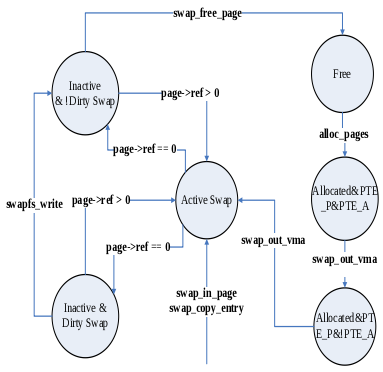
\includegraphics{figures/3.png} 图 页目录表和页表构成的二级页表映射架构

从图中可见,控制寄存器CR3的内容是对应页目录表的物理基地址;页目录表可以指定1K个页表,这些页表可以分散存放在任意的物理页中,而不需要连续存放;每张页表可以指定1K个任意物理地址空间的页。存储页目录表和页表的基地址是按4KB对齐。当采用上述页表结构后,基于分页的线性地址到物理地址的转换过程如下图所示:

首先,CPU把控制寄存器CR3的高20位作为页目录表所在物理页的物理基地址,再把需要进行地址转换的线性地址的最高10位(即22\textasciitilde{}
31位)作为页目录表的索引,查找到对应的页目录表项,这个表项中所包含的高20位是对应的页表所在物理页的物理基地址;然后,再把线性地址的中间10位(即12\textasciitilde{}21位)作为页表中的页表项索引,查找到对应的页表项,这个表项所包含的的高20位作为线性地址的基地址(即页号)对应的物理地址的基地址(即页帧号);最后,把页帧号作为32位物理地址的高20位,把线性地址的低12位不加改变地作为32位物理地址的低12位,形成最终的物理地址。

如果每次访问内存单元都要访问位于内存中的页表,则访存开销太大。为了避免这类开销,x86
CPU把最近使用的地址映射数据存储在其内部的页转换高速缓存(页转换查找缓存,简称TLB)中。这样在访问存储器页表之前总是先查阅高速缓存,仅当必须的转换不在高速缓存中时,才访问存储器中的两级页表。

\section{【实现】实现分页内存管理}\label{ux5b9eux73b0ux5b9eux73b0ux5206ux9875ux5185ux5b58ux7ba1ux7406}

\subsection{重新建立段映射}\label{ux91cdux65b0ux5efaux7acbux6bb5ux6620ux5c04}

前面已经介绍了如何探测物理内存,接下来ucore需要根据物理内存的情况来建立分页管理机制。首先观察一下tools/kernel.ld文件在proj4.1和proj5中的区别,在proj4.1中:

\begin{lstlisting}
ENTRY(kern_init)

SECTIONS {
    /* Load the kernel at this address: "." means the current address */
    . = 0x100000;

    .text : {
        *(.text .stub .text.* .gnu.linkonce.t.*)
    }
\end{lstlisting}

在porj5中:

\begin{lstlisting}
ENTRY(kern_entry)

SECTIONS {
    /* Load the kernel at this address: "." means the current address */
    . = 0xC0100000;

    .text : {
        *(.text .stub .text.* .gnu.linkonce.t.*)
    }
\end{lstlisting}

在意味着gcc编译出ucore的起始地址从0xC0100000开始,入口函数为kern\_entry函数。这与proj4.1有很大差别。这实际上说明ucore在建立好页映射关系后,虚拟地址空间和物理地址空间之间存在如下的映射关系:

\begin{lstlisting}
Virtual Address=LinearAddress=0xC0000000+Physical Address
\end{lstlisting}

另外,ucore的入口地址也改为了kern\_entry函数,这个函数位于init/entry.S中,分析代码可以看出,entry.S重新建立了段映射关系,从以前的

\begin{lstlisting}
Virtual Address= Linear Address
\end{lstlisting}

改为

\begin{lstlisting}
Virtual Address=Linear Address-0xC0000000
\end{lstlisting}

由于gcc编译出的虚拟起始地址从0xC0100000开始,ucore被bootloader放置在从物理地址0x100000处开始的物理内存中。所以当kern\_entry函数完成新的段映射关系后,且ucore在没有建立好页映射机制前,CPU按照ucore中的虚拟地址执行,能够被分段机制映射到正确的物理地址上,确保ucore运行正确。

\subsection{初始化物理内存页分配管理}\label{ux521dux59cbux5316ux7269ux7406ux5185ux5b58ux9875ux5206ux914dux7ba1ux7406}

为了与以后的分页机制配合,我们首先需要建立对整个计算机的页级物理内存分配管理。这部分代码的实现在kern/default\_pmm.{[}ch{]}。首先我们需要用一个数据结构来描述每个物理页(也称页帧),这里用了双向链表结构来表示每个页。链表头用free\_area\_t结构来表示,包含了一个list\_entry结构的双向链表指针和记录当前空闲页的个数的无符号整型变量nr\_free。

\begin{lstlisting}
/* free_area_t - maintains a doubly linked list to record free (unused) pages */
typedef struct {
    list_entry_t free_list;         // the list header
    unsigned int nr_free;           // # of free pages in this free list
} free_area_t;
\end{lstlisting}

每一个物理页的属性用结构Page来表示,它包含了映射此物理页的虚拟页个数,描述物理页属性的flags和双向链接各个Page结构的page\_link双向链表。

\begin{lstlisting}
struct Page {
    atomic_t ref;   // page frame's reference counter
    uint32_t flags; // array of flags that describe the status of the page frame
    list_entry_t page_link; // free list link
};
\end{lstlisting}

有了这两个数据结构,ucore就可以管理起来整个以页为单位的物理内存空间。接下来需要解决两个问题:
* 管理页级物理内存空间所需的Page结构的内存空间从哪里开始,占多大空间? *
空闲内存空间的起始地址在哪里?

对于这两个问题,我们首先根据bootloader给出的内存布局信息找出最大的物理内存地址maxpa(定义在page\_init函数中的局部变量),由于x86的起始物理内存地址为0,所以可以得知需要管理的物理页个数为

\begin{lstlisting}
npage = maxpa / PGSIZE
\end{lstlisting}

这样,我们就可以预估出管理页级物理内存空间所需的Page结构的内存空间所需的内存大小为:

\begin{lstlisting}
sizeof(struct Page) * npage)
\end{lstlisting}

由于bootloader加载ucore的结束地址(用全局指针变量end记录)以上的空间没有被使用,所以我们可以把end按页大小为边界去整后,作为管理页级物理内存空间所需的Page结构的内存空间,记为:

\begin{lstlisting}
pages = (struct Page *)ROUNDUP((void *)end, PGSIZE);
\end{lstlisting}

为了简化起见,从地址0到地址pages+ sizeof(struct Page) *
npage)结束的物理内存空间设定为已占用物理内存空间(起始0\textasciitilde{}640KB的空间是空闲的),地址pages+
sizeof(struct Page) *
npage)以上的空间为空闲物理内存空间,这时的空闲空间起始地址为

\begin{lstlisting}
uintptr_t freemem = PADDR((uintptr_t)pages + sizeof(struct Page) * npage);
\end{lstlisting}

为此我们需要把这两部分空间给标识出来。对于已占用物理空间,通过如下语句即可实现占用标记:

\begin{lstlisting}
for (i = 0; i < npage; i ++) {
    SetPageReserved(pages + i);
}
\end{lstlisting}

对于空闲物理空间,通过如下语句即可实现空闲标记:

\begin{lstlisting}
//获得空闲空间的起始地址begin和结束地址end
……
init_memmap(pa2page(begin), (end - begin) / PGSIZE);
\end{lstlisting}

其实SetPageReserved只需把物理地址对应的Page结构中的flags标志设置为PG\_reserved
,表示这些页已经被使用了。而init\_memmap函数则是把空闲物理页对应的Page结构中的flags和引用计数ref清零,并加到free\_area.free\_list指向的双向列表中,为将来的空闲页管理做好初始化准备工作。

\subsection{物理内存页分配与释放}\label{ux7269ux7406ux5185ux5b58ux9875ux5206ux914dux4e0eux91caux653e}

关于内存分配的操作系统原理方面的知识有很多,但在proj5中只实现了最简单的内存页分配算法,即每次只分配一页或释放一页的内存页分配算法。相应的实现在default\_pmm.c中的default\_alloc\_pages函数和default\_free\_pages函数,相关实现很简单,这里就不具体分析了,直接看源码,应该很好理解。

其实proj5在内存分配和释放方面最主要的作用是建立了一个物理内存页管理器框架,这实际上是一个函数指针列表,定义如下:

\begin{lstlisting}
struct pmm_manager {
    const char *name; //物理内存页管理器的名字
    void (*init)(void); //初始化内存管理器
    void (*init_memmap)(struct Page *base, size_t n); //初始化管理空闲内存页的数据结构
    struct Page *(*alloc_pages)(size_t n); //分配n个物理内存页
    void (*free_pages)(struct Page *base, size_t n); //释放n个物理内存页
    size_t (*nr_free_pages)(void); //返回当前剩余的空闲页数
    void (*check)(void); //用于检测分配/释放实现是否正确的辅助函数
};
\end{lstlisting}

重点是实现init\_memmap/ alloc\_pages/
free\_pages这三个函数。当完成物理内存页管理初始化工作后,计算机系统的内存布局如下图所示:

\begin{figure}[htbp]
\centering
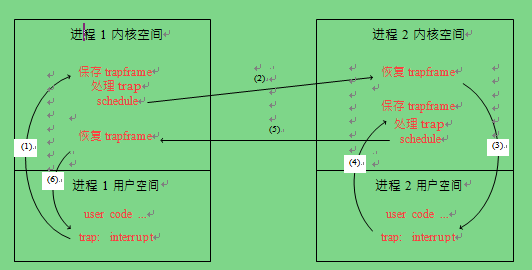
\includegraphics{figures/4.png}
\caption{4}
\end{figure}

\lstinline!chapt3-proj5-memory.vsd!

读者可进一步通过分析proj5.1/5.1.1/5.1.2/5.2中firstfit\_pmm{[}ch{]}/bestfit\_pmm{[}ch{]}/
worstfit\_pmm{[}ch{]}/
buddy\_pmm{[}ch{]}文件中对应函数实现来体会原理课中的连续空间内存分配中各种分配算法的设计思路和实现。

\subsection{建立二级页表}\label{ux5efaux7acbux4e8cux7ea7ux9875ux8868}

为了实现分页机制,需要建立好虚拟内存和物理内存的页映射关系,即建立二级页表。这需要解决如下问题:
* 对于哪些物理内存空间需要建立页映射关系? * 具体的页映射关系是什么? *
页目录表的起始地址设置在哪里? *
页表的起始地址设置在哪里,需要多大空间? * 如何设置页目录表项的内容? *
如何设置页目录表项的内容?

下面我们逐一解决上述问题。由于物理内存页管理器管理了从0到实际可用物理内存大小的物理内存空间,所以对于这些物理内存空间都需要建立好页映射关系。由于目前ucore只运行在内核空间,所以可以建立一个一一映射关系。假定虚拟内核地址的起始地址为0xC0000000,这虚拟内存和物理内存的具体页映射关系为:

\begin{lstlisting}
Virtual Address=Physical Address+0xC0000000 
\end{lstlisting}

由于我们已经具有了一个物理内存页管理器default\_pmm\_manager,我们就可以用它来获得所需的空闲物理页。在二级页表结构中,页目录表占4KB空间,ucore就可通过default\_pmm\_manager的default\_alloc\_pages函数获得一个空闲物理页,这个页的起始物理地址就是页目录表的起始地址。同理,ucore也通过这种方式获得各个页表所需的空间。页表的空间大小取决与页表要管理的物理页数n,一个页表项(32位,即4字节)可管理一个物理页,页表需要占n/256个物理页空间。这样页目录表和页表所占的总大小为4096+1024*n字节。

为把0\textasciitilde{}KERNSIZE(明确ucore设定实际物理内存不能超过KERNSIZE值,即0x38000000字节,896MB,3670016个物理页)的物理地址一一映射到页目录表项和页表项的内容,其大致流程如下:

\begin{enumerate}
\def\labelenumi{\arabic{enumi}.}
\item
  先通过default\_pmm\_manager获得一个空闲物理页,用于页目录表;
\item
  调用boot\_map\_segment函数建立一一映射关系,具体处理过程以页为单位进行设置,即
  Virtual Address=Physical Address+0xC0000000

  \begin{itemize}
  \item
    设一个逻辑地址la(按页对齐,故低12位为零)对应的物理地址pa(按页对齐,故低12位为零),如果在页目录表项(la的高10位为索引值)中的存在位(PTE\_P)为0,表示缺少对应的页表空间,则可通过default\_pmm\_manager获得一个空闲物理页给页表,页表起始物理地址是按4096字节对齐的,这样填写页目录表项的内容为

    页目录表项内容 = 页表起始物理地址\textbar{} PTE\_U \textbar{} PTE\_W
    \textbar{} PTE\_P
  \item
    进一步对于页表中对应页表项(la的中10位为索引值)的内容为 页表项内容
    = pa \textbar{} PTE\_P \textbar{} PTE\_W 其中:

    \begin{itemize}
    \item
      PTE\_U:位3,表示用户态的软件可以读取对应地址的物理内存页内容
    \item
      PTE\_W:位2,表示物理内存页内容可写
    \item
      PTE\_P:位1,表示物理内存页存在
    \end{itemize}
  \end{itemize}
\end{enumerate}

建立好一一映射的二级页表结构后,接下来就要使能分页机制了,这主要是通过enable\_paging函数实现的,这个函数主要做了两件事:

\begin{itemize}
\item
  通过lcr3指令把页目录表的起始地址存入CR3寄存器中;
\item
  通过lcr0指令把cr0中的CR0\_PG标志位设置上。
\end{itemize}

执行完enable\_paging函数后,计算机系统进入了分页模式!但到这一步还不够,还记得ucore在最开始通过kern\_entry函数设置了临时的新段映射机制吗?这个临时的新段映射机制不是最简单的对等映射,导致虚拟地址和线性地址不相等。而刚才建立的页映射关系是建立在简单的段对等映射,即虚拟地址=线性地址的假设基础之上的。所以我们需要进一步调整段映射关系,即重新设置新的GDT,建立对等段映射。

这里需要注意:在进入分页模式到重新设置新GDT的过程是一个过渡过程。在这个过渡过程中,已经建立了页表机制,所以通过现在的段机制和页机制实现的地址映射关系为:

\begin{lstlisting}
Virtual Address=Linear Address + 0xC0000000 = Physical Address +0xC0000000+0xC0000000
\end{lstlisting}

在这个特殊的阶段,如果不把段映射关系改为Virtual Address = Linear
Address,则通过段页式两次地址转换后,无法得到正确的物理地址。为此我们需要进一步调用gdt\_init函数,根据新的gdt全局段描述符表内容(gdt定义位于pmm.c中),恢复以前的段映射关系,即使得Virtual
Address = Linear
Address。这样在执行完gdt\_init后,通过的段机制和页机制实现的地址映射关系为:

\begin{lstlisting}
Virtual Address=Linear Address = Physical Address +0xC0000000
\end{lstlisting}

这里存在的一个问题是,在调用enable\_page函数使能分页机制后到执行完毕gdt\_init函数重新建立好段页式映射机制的过程中,内核使用的还是旧的段表映射,也就是说,enable
paging 之后,内核使用的是页表的低地址 entry。
如何保证此时内核依然能够正常工作呢?其实只需让低地址目录表项的内容等于以KERNBASE开始的高地址目录表项的内容即可。目前内核大小不超过
4M (实际上是3M,因为内核从 0x100000
开始编址),这样就只需要让页表在0\textasciitilde{}4MB的线性地址与KERNBASE
\textasciitilde{} KERNBASE+4MB的线性地址获得相同的映射即可,都映射到
0\textasciitilde{}4MB
的物理地址空间,具体实现在pmm.c中pmm\_init函数的语句:

\begin{lstlisting}
boot_pgdir[0] = boot_pgdir[PDX(KERNBASE)];
\end{lstlisting}

实际上这种映射也限制了内核的大小。当内核大小超过预期的3MB
就可能导致打开分页之后内核
crash,在后面的试验中,也的确出现了这种情况。解决方法同样简单,就是拷贝更多的高地址项到低地址。

当执行完毕gdt\_init函数后,新的段页式映射已经建立好了,上面的0\textsubscript{4MB的线性地址与0}4MB的物理地址一一映射关系已经没有用了。所以可以通过如下语句解除这个老的映射关系。

\begin{lstlisting}
boot_pgdir[0] = 0;
\end{lstlisting}

\subsection{自映射机制}\label{ux81eaux6620ux5c04ux673aux5236}

上一小节讲述了通过boot\_map\_segment函数建立了基于一一映射关系的页目录表项和页表项,这里的映射关系为:

\begin{lstlisting}
Virtual addr (KERNBASE~KERNBASE+KMEMSIZE) = Physical_addr (0~KMEMSIZE)
\end{lstlisting}

这样只要给出一个虚地址和一个物理地址,就可以设置相应PDE和PTE,就可完成正确的映射关系。

如果我们这时需要按虚拟地址的地址顺序显示整个页目录表和页表的内容,则要查找页目录表的页目录表项内容,根据页目录表项内容找到页表的物理地址,再转换成对应的虚地址,然后访问页表的虚地址,搜索整个页表的每个页目录项。这样过程比较繁琐。我们有没有一个简洁的方法来实现这个查找呢?ucore做了一个很巧妙的地址自映射设计,把页目录表和页表放在一个连续的4MB虚拟地址空间中,并设置页目录表自身的虚地址\textless{}--\textgreater{}物理地址映射关系。这样在已知页目录表起始虚地址的情况下,通过连续扫描这特定的4MB虚拟地址空间,就很容易访问每个页目录表项和页表项内容。

具体而言,ucore是这样设计的,首先设置了一个常量(memlayout.h):

\begin{lstlisting}
VPT=0xFAC00000, 
\end{lstlisting}

这个地址的二进制表示为:

\begin{lstlisting}
1111 1010 1100 0000 0000 0000 0000 0000
\end{lstlisting}

高10位为1111 1010
11,即10进制的1003,中间10位为0,低12位也为0。在pmm.c中有两个全局初始化变量

\begin{lstlisting}
pte_t * const vpt = (pte_t *)VPT;
pde_t * const vpd = (pde_t *)PGADDR(PDX(VPT), PDX(VPT), 0);
\end{lstlisting}

NaN. 并在pmm\_init函数执行了如下语句:

\begin{lstlisting}
boot_pgdir[PDX(VPT)] = PADDR(boot_pgdir) | PTE_P | PTE_W;
\end{lstlisting}

这些变量和语句有何特殊含义呢?其实vpd变量的值就是页目录表的起始虚地址0xFAFEB000,且它的高10位和中10位是相等的,都是10进制的1003。当执行了上述语句,就确保了vpd变量的值就是页目录表的起始虚地址,且vpt是页目录表中第一个目录表项指向的页表的起始虚地址。此时描述内核虚拟空间的页目录表的虚地址为0xFAFEB000,大小为4KB。页表的理论连续虚拟地址空间0xFAC00000\textasciitilde{}0xFB000000,大小为4MB。因为这个连续地址空间的大小为4MB,可有1M个PTE,即可映射4GB的地址空间。

但ucore实际上不会用完这么多项,在memlayout.h中定义了常量

\begin{lstlisting}
#define KMEMSIZE            0x38000000
\end{lstlisting}

表示ucore只支持896MB的物理内存空间,这个896MB只是一个设定,可以根据情况改变。则最大的内核虚地址为常量

\begin{lstlisting}
\#define KERNTOP             (KERNBASE + KMEMSIZE)=0xF8000000
\end{lstlisting}

所以最大内核虚地址KERNTOP的页目录项虚地址为

\begin{lstlisting}
vpd+0xF8000000/0x400000=0xFAFEB000+0x3E0=0xFAFEB3E0
\end{lstlisting}

最大内核虚地址KERNTOP的页表项虚地址为:
vpt+0xF8000000/0x1000=0xFAC00000+0xF8000=0xFACF8000

在pmm.c中的函数print\_pgdir就是基于ucore的页表自映射方式完成了对整个页目录表和页表的内容扫描和打印。注意,这里不会出现某个页表的虚地址与页目录表虚地址相同的情况。

自映射机制还可方便用户态程序访问页表。因为页表是内核维护的,用户程序很难知道自己页表的映射结构。VPT
实际上在内核地址空间的,我们可以用同样的方式实现一个用户地址空间的映射(比如
pgdir{[}UVPT{]} = PADDR(pgdir) \textbar{} PTE\_P \textbar{}
PTE\_U,注意,这里不能给写权限,并且 pgdir 是每个进程的 page table,不是
boot\_pgdir),这样,用户程序就可以用和内核一样的 print\_pgdir
函数遍历自己的页表结构了。

在page\_init函数建立完实现物理内存一一映射和页目录表自映射的页目录表和页表后,一旦使能分页机制,则ucore看到的内核虚拟地址空间如下图所示:

\begin{figure}[htbp]
\centering
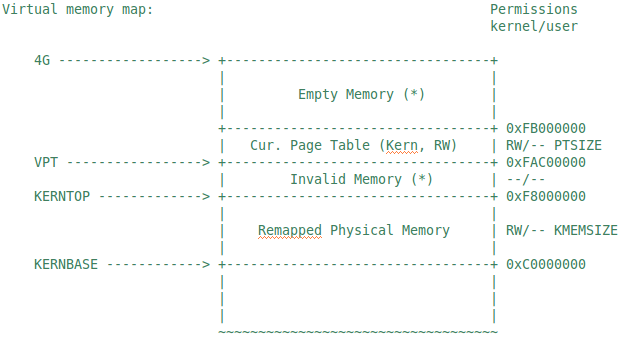
\includegraphics{figures/5.png}
\caption{5}
\end{figure}

proj5使能分页机制后的虚拟地址空间图

\section{【原理】页内存分配算法}\label{ux539fux7406ux9875ux5185ux5b58ux5206ux914dux7b97ux6cd5}

在proj5中进行在动态分配内存时,存在很多限制,效率很低。在操作系统原理中,为了有效地分配内存,首先需要了解和跟踪空闲内存和分布情况,一般可采用位图(bit
map)和双向链表两种方式跟踪内存使用情况。若采用位图方式,则每个页对应位图区域的一个bit,如果此位为0,表示空闲,如果为1,表示被占用。采用位图方式很省空间,但查找n个长度为0的位串的开销比较大。而双向链表在查询或修改操作方面灵活性和效率较高,所以ucore采用双向链表来跟踪跟踪内存使用情况。

假设整个物理内存空闲空间的以页为单位被一个双向链表管理起来,每个表项管理一个物理页。这需要设计某种算法来查找空闲页和回收空闲页。ucore实现了首次适配(first
fit)算法、最佳适配(best fit)算法、最差适配(worst
fit)算法和兄弟(buddy)算法,这些算法都可以实现在ucore提供的物理内存页管理器框架pmm\_manager下。

首次适配(first
fit)算法的分配内存的设计思路是物理内存页管理器顺着双向链表进行搜索空闲内存区域,直到找到一个足够大的空闲区域,这是一种速度很快的算法,因为它尽可能少地搜索链表。如果空闲区域的大小和申请分配的大小正好一样,则把这个空闲区域分配出去,成功返回;否则将该空闲区分为两部分,一部分区域与申请分配的大小相等,把它分配出去,剩下的一部分区域形成新的空闲区。其释放内存的设计思路很简单,只需把这块区域重新放回双向链表中即可。

最佳适配(best
fit)算法的设计思路是物理内存页管理器搜索整个双向链表(从开始到结束),找出能够满足申请分配的空间大小的最小空闲区域。找到这个区域后的处理以及释放内存的处理与上面类似。最佳适配算法试图找出最接近实际需要的空闲区,名字上听起来很好,其实在查询速度上较慢,且较易产生多的内存碎片。

最差适配(worst fit)算法与最佳适配(best
fit)算法的设计思路相反,物理内存页管理器搜索整个双向链表,找出能够满足申请分配的空间大小的最大空闲区域,使新的空闲区比较大从而可以继续使用。在实际效果上,查询速度上也较慢,产生内存碎片相对少些。

上述三种算法在实际应用中都会产生碎片较多,效率不高的问题。为此一般操作系统会采用buddy算法来改进上述问题。buddy算法的基本设计思想是:在buddy系统中,被占用的内存空间和空闲内存空间的大小均为2的k次幂(k是正整数)。这样在ucore中,若申请n个页的内存空间,则实际可能分配的空间大小为2K个页(2k-1\textless{}n\textless{}=2k)。若初始化时的空闲内存空间容量为2m个页,这空闲块的大小只可能是20、21、\ldots{}、2m个页。

\begin{figure}[htbp]
\centering
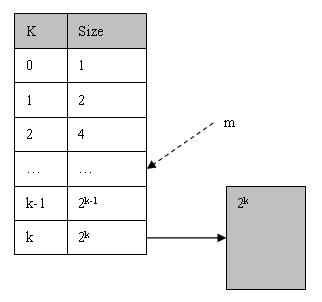
\includegraphics{figures/6.png}
\caption{6}
\end{figure}

假定内存一开始是一个连续地址空间(大小为2\^{}k个页)的大空闲块,且最小分配单位为1个页(4KB),则buddy
system初始化时将生成一个长度为k + 1的可用空间表List,
并将全部可用空间作为一个大小为2\^{}k个页的空闲块Bk挂接在空闲块数组链表List的最后一个节点上,
如下图:

\begin{figure}[htbp]
\centering
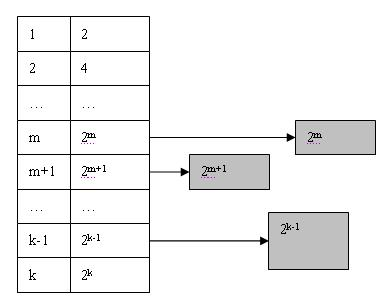
\includegraphics{figures/7.png}
\caption{7}
\end{figure}

当ucore其他子系统申请n个字节的存储空间时, buddy
system分配的空闲块大小为2\^{} m个页,m满足条件:2\^{} (m-1) \textless{}
n \textless{}= 2\^{} m

此时buddy
system将在list中的m位置寻找可用的空闲块。初始化时List中这个位置为空,
于是buddy system就向上查找m+1,\ldots{},直到达到k位置为止. 找到k位置后,
便得到可用空闲块Bk,
此时Bk将分裂成两个大小为2\^{}(k-1)的空闲块Bk-1a和Bk-1b,
并将其中一个插入到List中k-1位置, 同时对另外一个继续进行分裂.
如此以往直到得到两个大小为2\^{}m个页的块为止,并把其中一个空闲块分配给需求方。此时的内存如下图所示:

\begin{figure}[htbp]
\centering
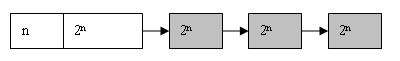
\includegraphics{figures/8.png}
\caption{8}
\end{figure}

如果buddy system在运行一段时间之后, List中某个位置t可能会出现多个块,
则将其他块依次链接可用块链表的末尾。当buddy system要在t位置取可用块时,
直接从链表头取一个即可。

当一个存储块被释放时, buddy
system将把此内存块回收到空闲块链表List中。此时buddy
system系统将根据此存储块的大小计算出其在List中的位置,
然后插入到空闲块链表的末尾。在这一步完成后, 系统立即开始合并尝试操作,
该操作是将地址相邻且大小相等的空闲块(简称buddy,即``伙伴''空闲块)合并到一起,
形成一个更大的空闲块,并重新放到空闲块链表List的对应位置中,
并继续对更大的块进行合并, 直到无法合并为止。

严蔚敏老师的``数据结构''一书第8章第4节对buddy算法有详尽的解释,``understanding
linux kernel''此书对此也有很好的描述,读者可以进一步参考。

对于上述4个内存分配算法,可参考对应的proj5.1/5.1.1/5.1.2/5.2中的kern/mm/*\_pmm.{[}ch{]}的具体实现来进一步了解。

\lstinline!(可以进一步描述三种算法的具体实现)!

\section{支持任意大小内存分配}\label{ux652fux6301ux4efbux610fux5927ux5c0fux5185ux5b58ux5206ux914d}

\subsection{试验目标}\label{ux8bd5ux9a8cux76eeux6807}

上一节描述了如何进行页级内存的分配与释放管理,可以比较有效地完成以页大小为最小单位(粒度)的内存分配和回收工作,这样可以很好地与分页机制配合在一起提供有效的分页管理。但在操作系统的实际运行过程中,还有很多对小于一页的任意大小内存的动态申请需求,则以页为最小单位就无法适应这类需求了。当然,我们可以直接把物理内存页管理器改为粒度为1字节的物理内存管理器,这主要存在两个问题:

\begin{itemize}
\tightlist
\item
  由于页目录表和页表的大小是4KB,且一个页表项管理的内存空间大小也是4KB,故需要扩展新的函数和结构匹配对页表的管理支持,导致代码复杂;
\item
  即使采用上述4种内存分配算法,在支持任意大小的内存分配请求上,依然存在效率不高,有外碎片和内碎片等问题。
\end{itemize}

所以,一个更加合理的办法是在物理内存页管理器的基础之上建立一个支持任意大小的内存分配管理器,形成二级内存管理,满足高效支持任意大小的内存分配请求。这就对动态内存分配管理提出了新的挑战,即花尽量少的时间完成对内存的分配和回收,且保证能够产生的内外碎片尽量小。

proj6中参考Jeff Bonwick 为 Sun OS
操作系统首次引入的一种算法:slab算法。slab算法的基本思路有两个,一个是通过缓存实现``对象''重用,另一个是在一个连续页空间放同样类型的``对象''。

Jeff Bonwick在SUN
OS内核中观察到内核在运行时会为有限的对象集(内核中各种常见的数据结构)分配大量内存,且对内核中这些数据结构进行初始化所需的时间超过了对其进行分配和释放所需的时间。因此他的结论是不应该将内存释放回一个全局的空闲内存池,而是将内存保持为针对特定目而初始化的状态。例如,如果内存被分配给了一个变量,那么只需在为此变量首次分配内存时执行一次变量初始化函数即可,当该变量被回收并进一步被后续分配时就不需要执行这个初始化函数,因为从上次释放和调用析构之后,它已经处于所需的状态中了。

在一个连续地址空间放同样类型的``对象''有助于快速查找和修改同样类型的``对象'',提高分配的时间效率,并减少碎片。

\subsection{proj6概述}\label{proj6ux6982ux8ff0}

\subsubsection{实现描述}\label{ux5b9eux73b0ux63cfux8ff0}

proj6基于proj5.2实现,主要在buddy物理内存页管理器的基础上,增加了一级任意大小内存分配管理,通过slab算法实现对小内存的简洁分配,为后续的运行时动态内存管理提供通用的内存申请和释放接口、在proj6中,可以了解到:

\begin{itemize}
\tightlist
\item
  slab算法的数据结构和具体实现;
\item
  小内存分配管理器与物理内存页管理器的接口和交互过程。
\end{itemize}

\subsubsection{项目组成}\label{ux9879ux76eeux7ec4ux6210}

\begin{lstlisting}
proj6
├── boot
│   └── ……
├── kern
│   ├── debug
│   │   └── ……
│   ├── driver
│   │   └── ……
│   ├── init
│   │   └── ……
│   ├── libs
│   │   └── ……
│   ├── mm
│   │   ├── ……
│   │   ├── memlayout.h
│   │   ├── slab.c
│   │   └── slab.h
│   ├── sync
│   │   └── ……
│   └── trap
│       └── ……
├── libs
│   └── ……
├── Makefile
└── ……

11 directories, 58 files
\end{lstlisting}

相对与proj5.2,proj6增加了slab.{[}ch{]}两个个文件,主要完成对slab内存管理算法的简单实现。

\subsubsection{编译运行}\label{ux7f16ux8bd1ux8fd0ux884c}

\begin{lstlisting}
(THU.CST) os is loading ...

Special kernel symbols:
  entry  0xc010002c (phys)
  etext  0xc0109530 (phys)
  edata  0xc0122aa0 (phys)
  end    0xc0123cb8 (phys)
Kernel executable memory footprint: 144KB
memory managment: buddy_pmm_manager
e820map:
  memory: 0009f400, [00000000, 0009f3ff], type = 1.
  memory: 00000c00, [0009f400, 0009ffff], type = 2.
  memory: 00010000, [000f0000, 000fffff], type = 2.
  memory: 07efd000, [00100000, 07ffcfff], type = 1.
  memory: 00003000, [07ffd000, 07ffffff], type = 2.
  memory: 00040000, [fffc0000, ffffffff], type = 2.
check_alloc_page() succeeded!
check_pgdir() succeeded!
check_boot_pgdir() succeeded!
-------------------- BEGIN --------------------
PDE(0e0) c0000000-f8000000 38000000 urw
  |-- PTE(38000) c0000000-f8000000 38000000 -rw
PDE(001) fac00000-fb000000 00400000 -rw
  |-- PTE(000e0) faf00000-fafe0000 000e0000 urw
  |-- PTE(00001) fafeb000-fafec000 00001000 -rw
--------------------- END ---------------------
check_slab() succeeded!
++ setup timer interrupts
100 ticks
100 ticks
\end{lstlisting}


\section{【实现】slab算法的简化设计实现}\label{ux5b9eux73b0slabux7b97ux6cd5ux7684ux7b80ux5316ux8bbeux8ba1ux5b9eux73b0}

\subsection{数据结构描述}\label{ux6570ux636eux7ed3ux6784ux63cfux8ff0}

slab 算法采用了两层数据组织结构。在最高层是
slab\_cache,这是一个不同大小slab
缓存的链接列表数组。slab\_cache的每个数组元素都是一个管理和存储给定大小的空闲对象(obj)的slab
结构链表,这样每个slab设定一个要管理的给定大小的对象池,占用物理空间连续的1个或多个物理页。slab\_cache的每个数组元素管理两种slab列表:

\begin{itemize}
\tightlist
\item
  slabs\_full:完全分配的 slab
\item
  slabs\_notfull:部分分配的 slab
\end{itemize}

注意 slabs\_notfull列表中的 slab 是可以进行回收(reaping),使得slab
所使用的内存可被返回给操作系统供其他子系统使用。

slab 列表中的每个 slab
都是一个连续的内存块(一个或多个连续页),它们被划分成一个个obj。这些obj是中进行分配和释放的基本元素。由于对象是从
slab 中进行分配和释放的,因此单个 slab 可以在 slab
链表之间进行移动。例如,当一个 slab 中的所有对象都被使用完时,就从
slabs\_notfull 链表中移动到 slabs\_full 链表中。当一个 slab
完全被分配并且有对象被释放后,就从 slabs\_full 列表中移动到
slabs\_notfull列表中。下面是ucore中的slab架构图:

\begin{figure}[htbp]
\centering
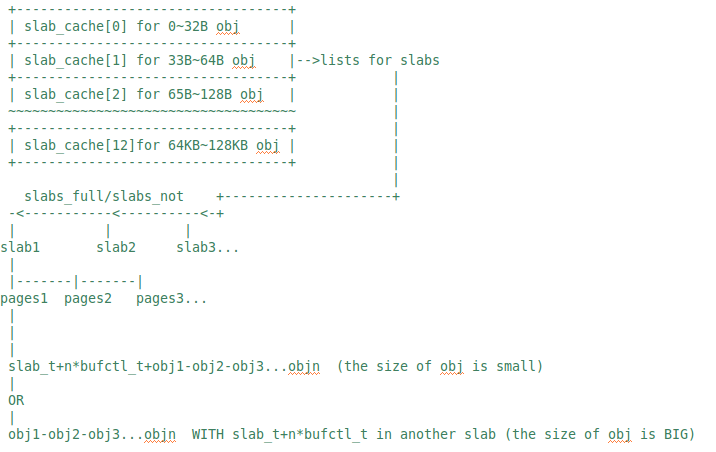
\includegraphics{figures/9.png}
\caption{8}
\end{figure}

slab架构图

\subsection{分配与释放内存实现描述}\label{ux5206ux914dux4e0eux91caux653eux5185ux5b58ux5b9eux73b0ux63cfux8ff0}

现在来看一下能够创建新 slab 缓存、向缓存中增加内存、销毁缓存的接口以及
slab 中对对象进行分配和释放操作的slab相关操作过程和函数。

第一个步骤是通过执行slab\_init函数初始化slab\_cache 缓存结构。然后其他
slab
缓存函数将使用该引用进行内存分配与释放等操作。ucore中最常用的内存管理函数是
kmalloc 和 kfree 函数。这两个函数的原型如下:

\begin{itemize}
\tightlist
\item
  void *kmalloc( size\_t size );
\item
  void kfree(void *objp );
\end{itemize}

在分配任意大小的空闲块时,kmalloc通过调用kmem\_cache\_alloc函数来遍历对应size的slab,来查找可以满足大小限制的缓存。如果kmem\_cache\_alloc函数发现slab中有空闲的obj,则分配这个对象;如果没有空闲的obj了,则调用kmem\_cache\_grow函数分配包含1到多页组成的空闲slab,然后继续分配。要使用
kfree
释放对象时,通过进一步调用kmem\_cache\_free把分配对象返回到slab中,并标记为空闲,建立空闲obj之间的链接关系。

\lstinline!(可进一步详细一些)!


%\input{}
%\input{}
%\input{}
%\input{}
%\input{}
%\input{}
%\input{}

\section{小结}
缺

